%============================================================
%  Silver Gjeka — Curriculum Vitae (English version)
%  Header Layout: Photo on Left, Name & Details on Right
%============================================================
\documentclass[a4paper,11pt]{article}

\usepackage[T1]{fontenc}
\usepackage[utf8]{inputenc}
\usepackage[english]{babel}
\usepackage{mathptmx}                 % Times-like font
\usepackage[top=0.7in,bottom=0.7in,left=0.85in,right=0.85in]{geometry}
\usepackage{enumitem}
\usepackage{tabularx}
\usepackage{graphicx}
\usepackage[hidelinks]{hyperref}

\pagestyle{empty}
\setlength{\parindent}{0pt}
\setlist[itemize]{leftmargin=1.4em,itemsep=1.5pt,topsep=2pt,parsep=0pt,label=\textbullet}

% ---- left-aligned small-caps section heading with rule ----
\newcommand{\cvsec}[1]{\vspace{7pt}{\large\scshape #1}\par\vspace{1.5pt}\hrule height 0.6pt\vspace{5pt}}

% ---- two-line entry: title (bold) + top-right / subtitle (italic) + bottom-right (italic) ----
\newcommand{\cventry}[4]{\textbf{#1}\hfill #2\par\textit{#3}\hfill\textit{#4}\par\vspace{1pt}}

% ---- compact project: name (bold) + stack (italic, right), description below ----
\newcommand{\proj}[3]{\textbf{#1}\hfill\textit{#3}\par #2\par\smallskip}

\begin{document}

%====================== HEADER (PHOTO ON LEFT, TEXT ON RIGHT) ======================
\noindent
\begin{minipage}[t]{0.22\textwidth}
  \vspace{0pt}
  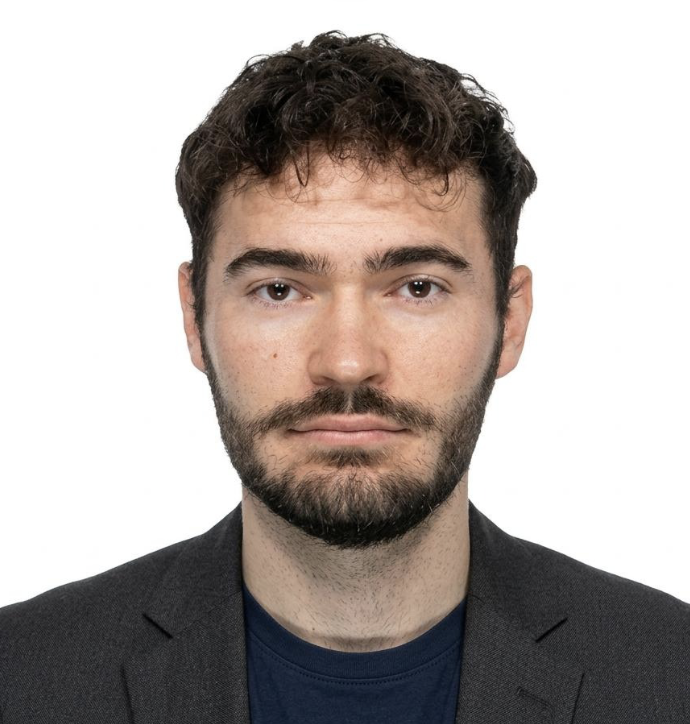
\includegraphics[width=3.1cm, height=3.6cm, keepaspectratio]{photo.png}
\end{minipage}%
\begin{minipage}[t]{0.78\textwidth}
  \vspace{0pt}
  \raggedright
  {\fontsize{24}{28}\selectfont\bfseries Silver Gjeka}\\[8pt]
  \begin{tabular}{@{}l@{\hspace{8pt}}l@{}}
    \textbf{Phone:}    & (+39) 351 6091609 \\[2pt]
    \textbf{Email:}    & \href{mailto:silvergjeka@gmail.com}{silvergjeka@gmail.com} \\[2pt]
    \textbf{GitHub:}   & \href{https://github.com/silvergjeka22}{github.com/silvergjeka22} \\[2pt]
    \textbf{LinkedIn:} & \href{https://www.linkedin.com/in/silver-gjeka-56b9931a4/}{linkedin.com/in/silver-gjeka-56b9931a4} \\[2pt]
    \textbf{Location:} & Verona, Italy
  \end{tabular}
\end{minipage}

\vspace{10pt}

%====================== SUMMARY ======================
\cvsec{Summary}

Artificial Intelligence master's student and Computer Science graduate at the University of Verona, specialized in machine learning, deep learning, computer vision and natural language processing, with a strong portfolio of hands-on AI projects. Backed by solid software-engineering and full-stack foundations, I build practical, data-driven AI systems end to end, from the model to the interface. Motivated, curious and eager to grow within an AI / machine-learning engineering team.

%====================== EDUCATION ======================
\cvsec{Education}

\cventry{University of Verona}{Verona, Italy}{M.Sc. in Artificial Intelligence}{2024 -- Present}
\begin{itemize}
  \item Focused on machine learning, deep learning, computer vision and natural language processing, combining strong theoretical foundations with hands-on AI projects. \textit{Final grade: in progress.}
\end{itemize}

\cventry{University of Verona}{Verona, Italy}{B.Sc. in Computer Science}{2020 -- 2024}
\begin{itemize}
  \item \textit{Thesis:} ``Development of a web app for monitoring IP uptime and security.''
\end{itemize}

%====================== EXPERIENCE ======================
\cvsec{Experience}

\cventry{Full Stack Developer}{2023 -- 2024}{BSQ}{Verona, Italy}
\begin{itemize}
  \item Designed and developed, end to end, a secure web application to monitor the uptime and security of IP devices (Bachelor's thesis), working independently across the full stack.
  \item Built asynchronous network scanning with Celery and Nmap (open-port detection, OS fingerprinting, security checks) with immediate threat notifications.
  \item Developed an interactive dashboard with map geolocation, real-time up/down monitors and a searchable device table.
  \item Implemented secure authentication, role-based permissions (user/admin) and multi-language support, backed by a MySQL database.
  \item Stack: Python, Flask, Django, Celery, Nmap, MySQL, HTML, CSS, JavaScript, Bootstrap.
\end{itemize}

\cventry{Barman}{Jun 2022 -- Sep 2022}{Compass Group}{Verona, Italy}
\begin{itemize}
  \item Customer service in a fast-paced environment; strengthened communication, teamwork and time management.
\end{itemize}

%====================== TECHNICAL SKILLS ======================
\cvsec{Technical Skills}

\textbf{AI / ML:} PyTorch, scikit-learn, Hugging Face Transformers, Computer Vision, Deep Learning, NLP, Reinforcement Learning, Explainable AI \\[3pt]
\textbf{Languages:} Python, Java, C, JavaScript, Swift, MATLAB \\[3pt]
\textbf{Web:} Flask, Django, HTML, CSS, Bootstrap \\[3pt]
\textbf{Data \& Tools:} MySQL, pandas, NumPy, Celery, Nmap, Git/GitHub, LaTeX \\[3pt]
\textbf{Spoken:} Albanian (Native), Italian (C1), English (B2)

%====================== PROJECTS ======================
\cvsec{Projects}

\proj{Bone Fracture Detection with Explainable AI}{ResNet18 X-ray classifier whose Grad-CAM attention aligns with radiologists' annotations, with a YOLOv8 + classifier pipeline reaching 93\% accuracy.}{Python, PyTorch}
\proj{Visual Question Answering (VQA)}{Multimodal models that answer natural-language questions about images, comparing 8 vision--language architectures (CLIP, ResNet, BERT, LSTM).}{Python, PyTorch, Transformers}
\proj{Neuro-Symbolic Safe Driving}{Reinforcement-learning agents (DQN, PPO) made safer with traffic rules in temporal logic, cutting crashes from 35\% to 5\% in an unseen simulator.}{Python, RL}
\proj{Lifelong Action Learning}{Video action recognizer (CNN + LSTM) on UCF101 that learns new actions over time without forgetting, using replay, distillation and MAML meta-learning.}{Python, PyTorch}
\proj{MACURA Drone Racing}{Trained a simulated drone to race through a 3-D windy course, comparing model-based reinforcement-learning methods (MACURA, MBPO, M2AC, SAC).}{Python, MuJoCo}
\proj{Fitness Activity Recognition}{End-to-end ML pipeline classifying six gym exercises from accelerometer/gyroscope data; best model (Random Forest) reached 98.3\% accuracy.}{Python, scikit-learn}
\proj{CongruentClosureDAG}{DAG-based congruence-closure algorithm for the satisfiability of equality formulas with arrays, lists and uninterpreted functions, plus a graphical visualizer.}{Java}

\textbf{More projects:} explore the full AI \& software portfolio on \href{https://github.com/silvergjeka22}{github.com/silvergjeka22}.

%====================== AWARDS & TRAINING ======================
\cvsec{Awards \& Training}

\cventry{CyberChallenge.IT 2026}{Italy}{National cybersecurity training program}{2026}
\begin{itemize}
  \item Selected through a national competitive program covering network security, web application security, cryptography and ethical hacking.
\end{itemize}

\textbf{Open Badges:} iOS Development with Swift; Problem Solving \& Soft Skills (University of Verona, 2022).

\vspace{8pt}
{\footnotesize I authorize the processing of my personal data contained in this CV in accordance with EU Regulation 2016/679 (GDPR) and Italian Legislative Decree 196/2003.\par}

\vspace{18pt}
\begin{flushright}
{\itshape\Large Silver Gjeka}\\[6pt]
\rule{5.5cm}{0.4pt}\\
{\footnotesize Signature}
\end{flushright}

\end{document}
